\documentclass[12pt,a4paper,oneside]{report}
% nagyon sok kép esetén meggyorsítható a fordítás a draft móddal
% \documentclass[12pt,a4paper,oneside,draft]{report}
% ekkor a képek nem renderelődnek ki, csak placeholder lesz mérethelyesen
\usepackage[utf8]{inputenc} % mindenképp maradjon az utf-8 kódolás
\usepackage[magyar]{babel}
\usepackage[T1]{fontenc}
\usepackage{amsmath}
\usepackage{amsfonts}
\usepackage{amssymb}
\usepackage{graphics} % grafikus elemek, képek berakásához
\usepackage{epsfig} % eps importáláshoz
\usepackage{listings}
\usepackage{sectsty}
\usepackage{enumerate}
\usepackage{lastpage}
\usepackage{setspace}
\usepackage{hyperref} % PDF hivatkozásokhoz kell
\usepackage[hang]{caption}
\usepackage{titling} % a title, author parancsok szabad használatához
\usepackage{float}

\usepackage{listings}
\usepackage{color}

\definecolor{mygreen}{rgb}{0,0.6,0}
\definecolor{mygray}{rgb}{0.5,0.5,0.5}
\definecolor{mymauve}{rgb}{0.58,0,0.82}

\lstset{ 
  backgroundcolor=\color{white},   % choose the background color; you must add \usepackage{color} or \usepackage{xcolor}; should come as last argument
  basicstyle=\footnotesize,        % the size of the fonts that are used for the code
  breakatwhitespace=false,         % sets if automatic breaks should only happen at whitespace
  breaklines=true,                 % sets automatic line breaking
  captionpos=b,                    % sets the caption-position to bottom
  commentstyle=\color{mygreen},    % comment style
  deletekeywords={...},            % if you want to delete keywords from the given language
  escapeinside={\%*}{*)},          % if you want to add LaTeX within your code
  extendedchars=true,              % lets you use non-ASCII characters; for 8-bits encodings only, does not work with UTF-8
  firstnumber=1000,                % start line enumeration with line 1000
  frame=single,	                   % adds a frame around the code
  keepspaces=true,                 % keeps spaces in text, useful for keeping indentation of code (possibly needs columns=flexible)
  keywordstyle=\color{blue},       % keyword style
  language=Octave,                 % the language of the code
  morekeywords={*,...},            % if you want to add more keywords to the set
  numbers=left,                    % where to put the line-numbers; possible values are (none, left, right)
  numbersep=5pt,                   % how far the line-numbers are from the code
  numberstyle=\tiny\color{mygray}, % the style that is used for the line-numbers
  rulecolor=\color{black},         % if not set, the frame-color may be changed on line-breaks within not-black text (e.g. comments (green here))
  showspaces=false,                % show spaces everywhere adding particular underscores; it overrides 'showstringspaces'
  showstringspaces=false,          % underline spaces within strings only
  showtabs=false,                  % show tabs within strings adding particular underscores
  stepnumber=2,                    % the step between two line-numbers. If it's 1, each line will be numbered
  stringstyle=\color{mymauve},     % string literal style
  tabsize=2,	                   % sets default tabsize to 2 spaces
  title=\lstname                   % show the filename of files included with \lstinputlisting; also try caption instead of title
}

% a TikZ rajzoló modul, és a kapcsolási rajz készítő modul, ha kell
%\usepackage{tikz}
%\usepackage{circuitikz}

% az A4 oldal margóinak és méreteinek beállítása
\usepackage[left=25mm,right=25mm,top=20mm,bottom=25mm]{geometry}\pagestyle{plain}

% A sorköz távolság beállítása
% egyszeres sorköz
\singlespacing
% 1,5 sorköz
% \onehalfspacing

% A hivatkozások, és linkek átállítása alapértelmezett színre, fekete-fehér nyomtatáshoz optimalizálva
\hypersetup
{
  	colorlinks,
  	citecolor=black,
 	linkcolor=black,
  	urlcolor=black
}

% --------- A hallgató által kitöltendő rész! --------- %

% a dolgozat típusa
\title{Témalabor beszámoló} 

% a dolgozat szerzője
\author{dr. Dudás Levente}

% a dolgozat típusát adjuk meg tárgyesetben, kisbetűvel (pl.: diplomatervet, szakdolgozatot, témalabor beszámolót stb.)
\newcommand{\dokumentumtipus}{témalabor beszámolót} 

% a dolgozat témája
\newcommand{\dokumentumcim}{80m-es rádió iránymérő vevő és teszt adó}

% --------- A hallgató által kitöltendő rész! --------- %

\begin{document}
\begin{titlepage}

\begin{figure}
\centering

\includegraphics[width=100mm,keepaspectratio]{bme.pdf}
\end{figure}

\centering
\textbf{Budapesti Műszaki és Gazdaságtudományi Egyetem}\\
\textbf{Villamosmérnöki és Informatikai Kar}\\
\textbf{Szélessávú Hírközlés és Villamosságtan Tanszék}\\
\vspace{5mm}

\includegraphics[width=40mm,keepaspectratio]{hvt_logo_only_fixed_vector_inverted.png}  \\
\vspace{50mm}
\Huge
\dokumentumcim\\
\vspace{60mm}
\Large
\thetitle \\
\vspace{12mm}
\Large
\textbf{\theauthor}\\
\vspace{12mm}
\the\year


\end{titlepage}
%\newpage
\hspace{10mm}
\begin{center}
\large
\textbf{HALLGATÓI NYILATKOZAT}
\end{center}
\hspace{10mm}

Alulírott \theauthor, szigorló hallgató kijelentem, hogy ezt a \dokumentumtipus \ meg nem engedett segítség nélkül, saját magam készítettem, csak a megadott forrásokat (szakirodalom, eszközök stb.) használtam fel. Minden olyan részt, melyet szó szerint, vagy azonos értelemben, de átfogalmazva más forrásból átvettem, egyértelműen, a forrás megadásával megjelöltem.

Hozzájárulok, hogy a jelen munkám alapadatait (szerző(k), cím, angol és magyar nyelvű tartalmi kivonat, készítés éve, konzulens(ek) neve) a BME VIK nyilvánosan hozzáférhető elektronikus formában, a munka teljes szövegét pedig az egyetem belső hálózatán keresztül (vagy autentikált felhasználók számára) közzétegye. Kijelentem, hogy a benyújtott munka és annak elektronikus verziója megegyezik. Dékáni engedéllyel titkosított diplomatervek esetén a dolgozat szövege csak 3 év eltelte után válik hozzáférhetővé.

\hspace{10mm}

Budapest, \today

\begin{flushright}
\theauthor
\end{flushright}
% Ide kell include-olni, vagy befűzni a feladatkiírást, ha van
\tableofcontents
%\chapter*{Kivonat}

Jelen dokumentum egy diplomaterv sablon, amely formai keretet ad a BME Villamosmérnöki és Informatikai Karán végző hallgatók által elkészítendő szakdolgozatnak, és diplomatervnek. A sablon használata opcionális. Ez a sablon \LaTeX \  alapú, a TeXLive TeX 
implementációval és a PDF-LaTeX fordítóval működőképes.

%\chapter*{Abstract}

This document is ggg a \LaTeX -based template for the BSc/MSc thesis of students at the Electrical Engineering and Informatics Faculty of Budapest University of Technology and Economics. The usage of this template is optional. It has been tested with the TeXLive TEX implementation, and it requires the PDF-LaTeX compiler.
\chapter{Témalabor}

\section{Bevezetés}

A jelenleg zajló BSc képzésben, az önálló labort megelőző félévben Témalabort indítunk, mint ahogy az az előző félévi szakirány tájékoztatón is elhangzott.

Több más tanszékkel ellentétben (akik irodalomkutatást végeztetnek a hallgatókkal) mi a gyakorlatiasabb rész felé helyeznénk a hangsúlyt - többek között kedvcsinálónak illetve szintrehozónak szánva.

\section{A félév menete}

Ennek megfelelően a félév első felében - első 7 oktatási hét - mindegyik jelentkezett hallgató ugyanolyan áramkört épít meg dokumentáció és mérési utasítás alapján, az "Áramkörépítő szakkörös" pákákat illetve a "Lendületvételes" oszcilloszkópokat itt is hadrendbe állítva. \cite{hvthonlap}

A gyakorlati foglalkozások az első 7 oktatási héten, minden szerdán 8:15-12:00-ig lesznek megtartva a V1 épület 501/502 teremben. A megjelenés minden hallgatónak kötelező.

A félév második felében a hallgatók témakörök és laborok közül választhatnak, ahol egyéni vagy kisebb csoportokban a laborok által meghatározott feladatot kell elvégezniük.

Ezek a laborok és a hozzá tartozó oktatók, akiknél jelentkezni kell \aref{tab:laborok_es_oktatok} táblázatban láthatók.

\begin{table}[hb]
        \footnotesize
        \centering
        \caption{Oktatói táblázat}
        \begin{tabular}{ | l | l |}
        \hline
        Témakör & Oktató\\
        \hline
 		Antennák és EMC & dr. Nagy Lajos \\
 		DOCS & dr. Bitó János \\
 		EMT & dr. Pávó József \\
 		Mikrohullámú Távérzékelés & dr. Seller Rudolf \\
 		NES & Reichardt András \\
 		Űrtechnológia & dr. Csurgai-Horváth László \\
        \hline
        \end{tabular}
        \label{tab:laborok_es_oktatok}
\end{table}

\section{Követelmények}

\begin{enumerate}
\item
Az első 7 oktatási héten a gyakorlati foglalkozásokon a megjelenés kötelező, normál utcai viseletben.

Az áramkör előre gyártatott panelekre készül, kézi forrasztási eljárással (aki nem forrasztott még, az most megtanul), dokumentáció alapján.

Az egyes áramköri részegységek élesztése és bemérése (valamint mérés közbeni dokumentálása) az oktató kollégák segítségével történik digitális oszcilloszkópok felhasználásával.
\item
A félév második 7 hetes időszakában a hallgatók kisebb csoportokat alkotva egy-egy laborban tevékenykednek önállóan a laborok által meghatározott feladatokat elvégezve.

\item
A félév végén leadandó - a tanulmányi portálra feltöltendő - dokumentumok a következők:

\begin{itemize}
\item
A megadott sablon alapján készített mérési jegyzőkönyv a félév első felében épített áramkörről.
\item
5 - 10 oldal terjedelmű írásos beszámoló a félév második felében történt önálló munkáról csoportonként, a témát vezető oktató rövid értékelésével.
\item
A pótlási héten - felkészítve a hallgatókat a későbbi önálló labor beszámolókra, szakdolgozat illetve diplomaterv védésekre - 5 + 2 perces előadás jellegű beszámoló (LaTex pdf) a tárgyat hallgató hallgatók és az oktatók jelenlétében.
\end{itemize}

\end{enumerate}

A beszámolókhoz használható minta dokumentumok a következő linken érhetők el: \url{http://152.66.80.46/temalabor}

A félév végi érdemjegy a közös áramkör mérési jegyzőkönyve, a félév második felének írásos beszámolója és a félév pótlási hetében tartott 5 + 2 perces előadás alapján képződik egyenletes súlyozással 1-5-ig skálára kvantálva, ahol a \%-os határok a következők: 40, 55, 70, 85.

Például:
\begin{itemize}
\item
Mérési jegyzőkönyv: 85 \%
\item
Irásos beszámoló: 92 \%
\item
Előadás: 78 \%
\end{itemize}

Átlagban: (85+92+78)/3=85\% amely $\geq$ 85, vagyis jeles.



\chapter{Rókavevő}

\begin{enumerate}
\item
A rádió iránymérő vevő:\\
	Az egyes fokozatok a következők:
	\begin{itemize}
	\item 9 menetes (210 cm műanyag vagy lakk szigetelésű rézhuzalból) irányérzékeny keretantenna,
	\item rádiófrekvenciás erősítő,
	\item RF sáváteresztő szűrő,
	\item tranzisztoros keverő
	\item helyi oszcillátor,
	\item hangfrekvenciás alul áteresztő szűrő
	\item hangfrekvenciás erősítő.
	\end{itemize}
\item
A teszt adó:\\
	Collpitts típusú oszcillátor, amelyben a rezgőkvarc a vevőhöz képest néhány 100 Hz-cel el van hangolva, hogy a vétel oldalon a keverésnél előálljon egy különbségi hangfrekvenciás jel.
\end{enumerate}

\newpage
\section{Kapcsolási rajz}

A rókavevő kapcsolási rajza \aref{fig:rokasch}. ábrán látható.

\begin{figure}[H]
\centering
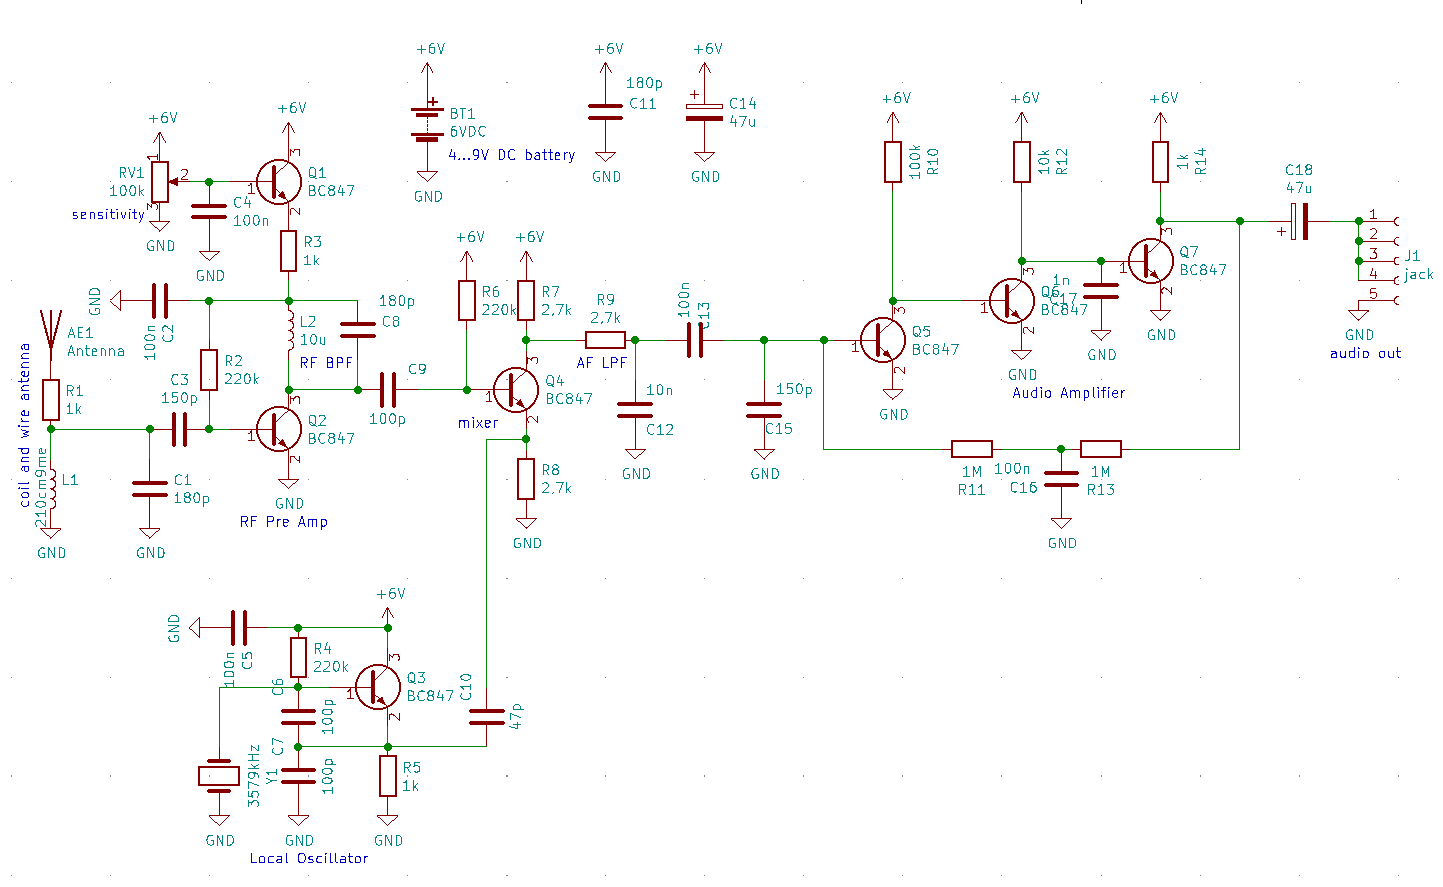
\includegraphics[width=1\textwidth]{../pic/sch.png}\\
\caption{A rókavevő kapcsolási rajza}
\label{fig:rokasch}
\end{figure}

\newpage
\section{Nyomtatott huzalozású lemez}

A NYHL egyoldalas, forrasztásgátló lakkal borított panel - \ref{fig:rokanyhl}. ábra, amely vegyesen furat- és felületszerelt alkatrészeket is tartalmaz.

\begin{figure}[H]
\centering
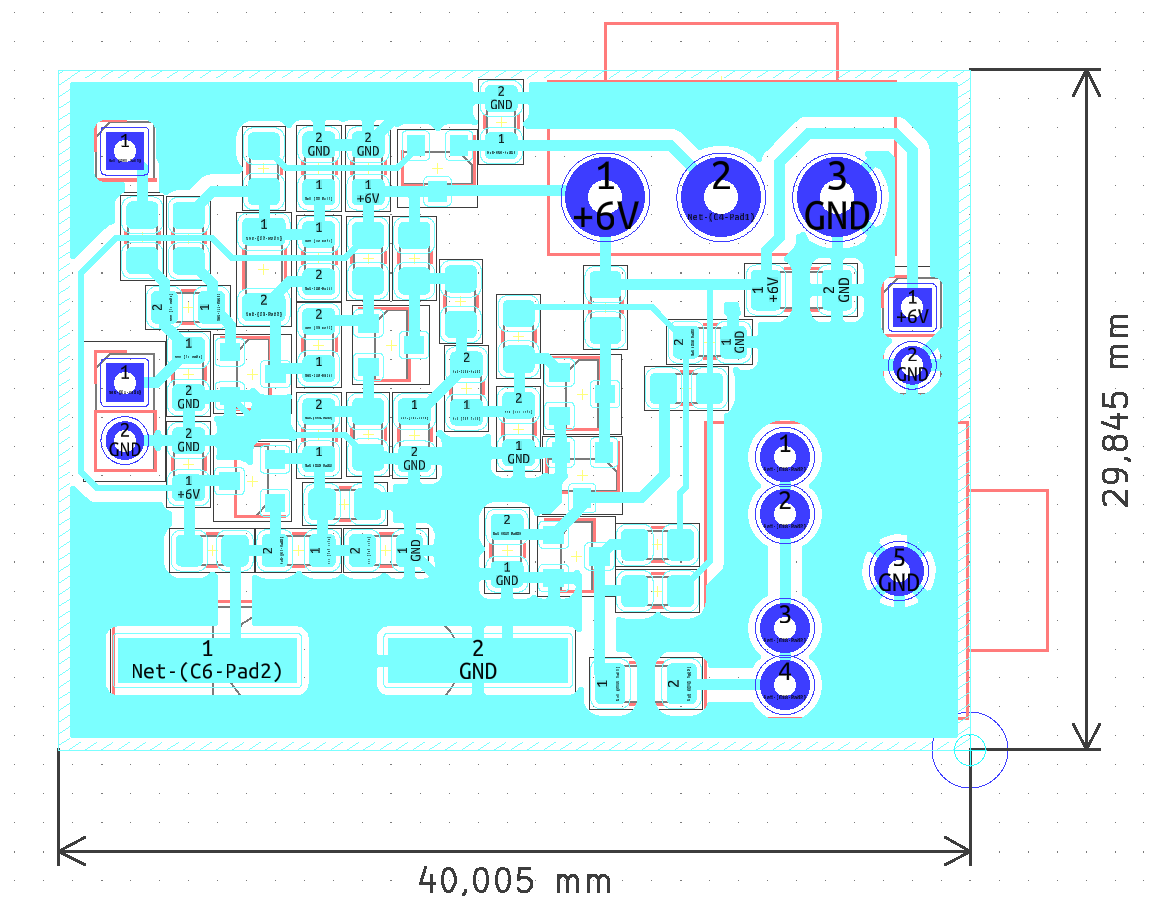
\includegraphics[width=1\textwidth]{../pic/pcb.png}
\caption{HYHL}
\label{fig:rokanyhl}
\end{figure}

\newpage
\section{Alkatrész ültetési rajz}

Az alkatrészek ültetési rajza - a különböző rétegekkel és feliratokkal - \aref{fig:rokault}. ábrán látható.

\begin{figure}[H]
\centering
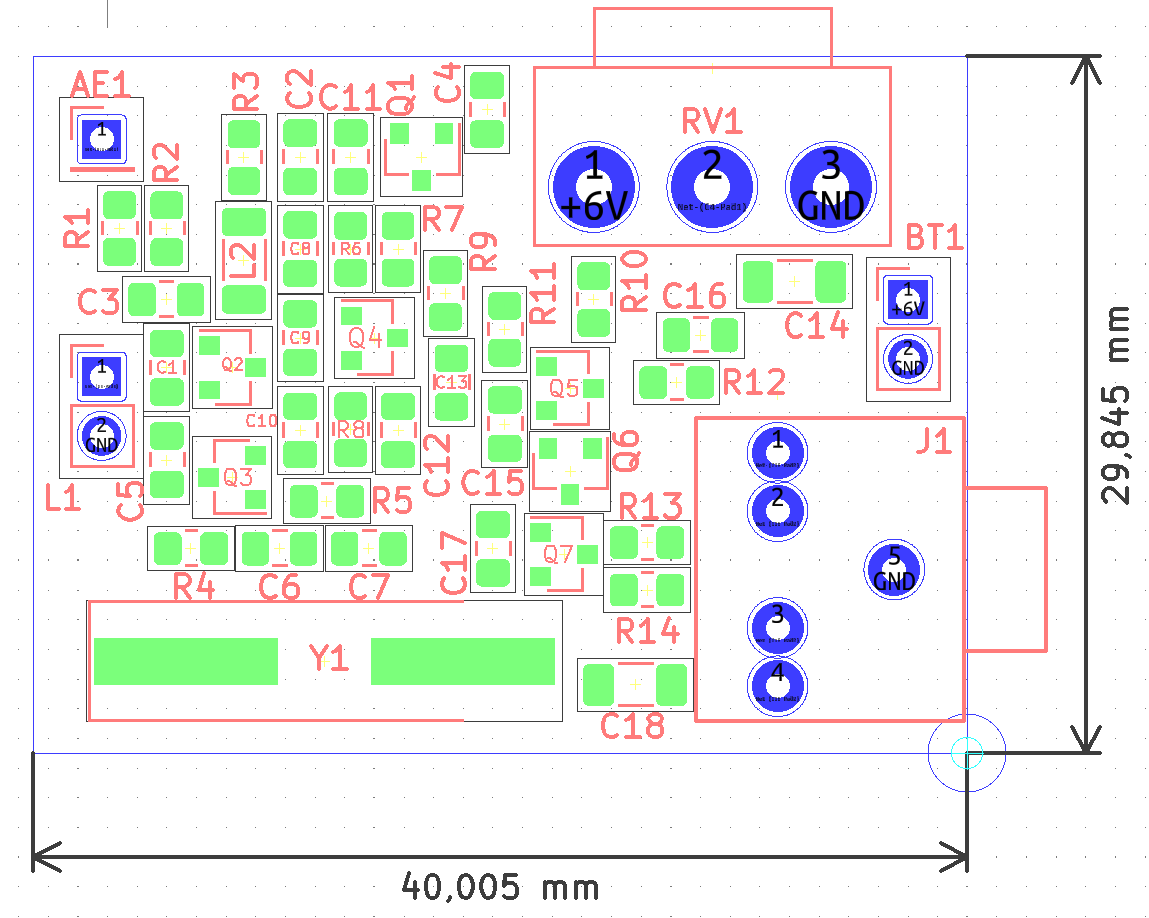
\includegraphics[width=1\textwidth]{../pic/pos.png}
\caption{Az alkatrészek elhelyezése}
\label{fig:rokault}
\end{figure}

Ültetési sorrend:

\begin{enumerate}
\item ellenállások,
\item kondenzátorok,
\item induktivitás (nem az antenna),
\item tranzisztorok,
\item csatlakozók,
\item antenna.
\end{enumerate}

\newpage
\section{Élesztés}

A rendelkezésre álló szárazelemekről indítva a vevő (hibátlan forrasztás esetén) azonnal működőképes.

\section{Mérési feladatok}

Oszcilloszkóp segítségével mérje meg a következőket:

\begin{enumerate}
\item Munkaponti DC feszültségek minden félvezető minden lábán a GND-hez (negatív telepcsatlakozási pont) képest.
\item Vevő helyi oszcillátor jelalak, $V_{pp}$, frekvencia az oszcillátor tranzisztor emitterén.
\item Vevő hangfrekis kimenet a jack csatlakozó meleg pontján a potméter min, közép és max. állásában: jelalak, $V_{pp}$ és frekvencia. - ekkor adott távolságból egy teszt adó fog üzemelni.
\end{enumerate}
\section{A mérési jegyzőkönyv formai követelményei}

\begin{itemize}
\item
A jegyzőkönyvben benne kell lennie, hogy mikor, milyen műszerrel történt a mérés (pl. a műszer gyári száma egyértelműen azonosítja a műszert) és ki vagy kik végezték a mérést.
\item
Minden logikailag összetartozó méréshez mérési elrendezési rajzot kell készíteni és rögzíteni kell az egyes beállított illetve mért paramétereket is. Ez azért szükséges, mert egy mérési jegyzőkönyv alapján reprodukálhatónak kell lennie a mérésnek, vagyis olyan részletességű kell legyen a mérési összeállítási rajz, hogy meg lehessen belőle állapítani, hogy melyik mérőponton, milyen beállítású mérőfejjel, hogyan történt a mérés.
\item
Minden mérési eredmény egyedileg vagy csoportosan röviden értékelni kell az adott részegységek paramétereinek megfelelően.
\item
A mérési összeállításról fényképfelvétel készítése is javasolt, amely helyettesítheti a mérési összeállítási rajzot, abban az esetben, ha minden eszköz illetve beállítás azon egyértelműen azonosítható.
\item
Ha valamilyen segédanyagot használtál (cikk, könyv, valakinek a diplomamunkája, Internetes segédanyag linkek, stb.), akkor azt az adott - logikailag megfelelő - helyen hivatkozd be, illetve tedd bele az irodalomjegyzék fájlba is. A Wikipédiás hivatkozások használatát mellőzd, ehelyett az ott hivatkozott irodalmat használd! - igaz ez mind a beszámolóra, mind a későbbi önlab doksikra, szakdolgozatokra és diplomatervekre egyaránt.
\end{itemize}

\subsection{A \LaTeX \ használatához további segítség}

Ha egy matematikai összefüggést kell leírnod (korrekt irodalmi hivatkozással \cite{diploma} ), akkor tedd például így: \ref{eq:antrow}.
% minden képlet esetén az align környzetet érdemes használni, mert ez a legújabb
\begin{align}
\ F ( \vartheta )= \sum_{k=0}^{N-1} I_k e^{-jk \beta d cos \vartheta} 
\label{eq:antrow}
\end{align}

Ahol:
\begin{itemize}
\item
$\vartheta$ a megfigyelési pont iránya az antennasorhoz képest
\item
$\beta$ a hullámszám (2$\pi$/$\lambda$)
\item
d az antennaelemek távolsága
\item
N az antennaelemek száma
\item
$I_k$ az aktuális antennaelem bemeneti komplex gerjesztése (árama)
\end{itemize}
Amennyiben kettő, vagy több egybe tartozó egyenletet kell leírni egyetlen környezetbe:
\begin{align}
\Delta \varphi &= 0 \\
\Delta \varphi &= -\frac{\varrho}{\varepsilon}
\end{align}
Az egyenlőség-jelhez igazított egyenleteket így lehet bevinni.
% Az '&' segítségével, oda rendezi az egymás felett levő egyenleteket, ahova az '&' jelet raktad.
% Figyelem! Az align környezet érzékeny az üres enterekre, ilyet ne hagyjunk, mert nem fordul a kód!
\\Ez itt egy függelék hivatkozás: \ref{fugg}

\subsection{Forráskódot}

például így társíthatsz LaTex-ben:

\lstinputlisting[language=C]{while1.c}
%\chapter*{Köszönetnyilvánítás}
Ide kerül az opcionális köszönetnyilvánítás, amelyben érdemes megemlíteni a konzulenst, illetve mindazokat, akik a dolgozat létrejöttében segítettek a szerzőnek. 
\begin{thebibliography}{4}

\bibitem{hvthonlap} \url{http://hvt.bme.hu}

\bibitem{radiotechnika} Rádiótechnika évkönyve 2007, 172. oldaltól

\bibitem{diploma} Dudás Levente, \emph{Digitális nyalábformálású antenna (DBF)} diplomaterv, BME SzHVT, 2007

\bibitem{kicad} \url{http://kicad-pcb.org/}

\end{thebibliography}


\listoffigures
\listoftables
\chapter*{Függelék}

A függelék az a fejezet, amely nem képezi szerves részét magának a dolgozatnak (nem növeli az oldalszámot), csak a megértést segíti, illetve a plusz ábrákat, pl. kapcsolási rajzokat, NYÁK terveket, program forráskódokat tartalmazza, de természetesen lehet hivatkozni rá (és sok esetben kell is). \label{fugg}

Jelen dokumentumot, nemcsak pdf, hanem \LaTeX \  forráskód szinten is közzéteszem, abból a megfontolásból, hogy lehetőség szerint legyen egységes a beadott beszámolók és jegyzőkönyvek formátuma és kinézete.

Jelen dokumentum forráskódja példákat tartalmaz a szövegek, képek, táblázatok, számozott és számozatlan felsorolások szerkesztésére, tagolására, formátumára vonatkozóan beleértve a matematika kifejezések forráskód szintű kezelését is.

A LaTeX letölthető többféle operációs rendszerre innen: 
\\
\url{https://www.latex-project.org/get/}

Ha valakinek magyar nyelvű szótárra van szüksége, akkor használhatja jelen dokumentum mappájában levő állományt is: a fordítóban kell beállítani a nyelvi beállításoknál.

% végső fordításnál kapcsold ki a draft módot !!

\end{document}